% Visual trial version — does not replace Group 7 slides.tex
% Compile: tectonic -X compile "Group 7 slides visual.tex"
\documentclass[aspectratio=169,12pt]{beamer}
\usepackage[T1]{fontenc}
\usepackage{lmodern}
\usepackage{amsmath,booktabs,graphicx,tikz}
\graphicspath{{visual-art/}{figures/}}
\definecolor{navy}{HTML}{1F3A5F}
\definecolor{accent}{HTML}{2F6690}
\setbeamercolor{structure}{fg=navy}
\setbeamercolor{title}{fg=navy}
\setbeamercolor{frametitle}{fg=navy}
\setbeamercolor{itemize item}{fg=accent}
\setbeamertemplate{navigation symbols}{}
\setbeamertemplate{itemize item}{\color{accent}\textbullet}
\setbeamertemplate{footline}{%
  \hfill{\scriptsize\color{navy!70}Group 7 \quad visual trial \quad \insertframenumber/\inserttotalframenumber\hspace{4mm}}}
\setbeamertemplate{frametitle}{\vspace{1.2mm}\insertframetitle\par\vspace{0.8mm}{\color{navy}\hrule height 0.7pt}\vspace{2mm}}
\setbeamerfont{frametitle}{series=\bfseries,size=\large}
\setbeamerfont{itemize/enumerate body}{size=\small}
\newcommand{\pe}{\pi_e}
\newcommand{\pb}{\pi_b}
\newcommand{\Vhat}{\widehat{V}}
\newcommand{\speak}[1]{\begin{itemize}\setlength{\itemsep}{0.42em}\setlength{\parskip}{0pt}#1\end{itemize}}
\newcommand{\art}[2][0.46\textwidth]{\includegraphics[width=#1,keepaspectratio]{#2}}
\begin{document}

\begin{frame}[plain]
\centering
\vspace{12mm}
{\color{navy}\LARGE\bfseries Offline Policy Evaluation\\[2mm] with Real-World Bandit Logs\par}
\vspace{9mm}
{\large Jingzhe FENG \quad Jun LI \quad Kaiwen WANG\\[2mm] Siyu YAN \quad Zenghuan WANG\par}
\vspace{8mm}
{\color{navy} Group 7 \quad City University of Hong Kong (Dongguan)\par}
\vspace{3mm}
{\small DSC6007 Dynamic Programming and Reinforcement Learning\\[1mm]
visual layout trial --- not the submission file}
\end{frame}

\begin{frame}{Why testing a new policy online is costly}
\begin{columns}[T]
\begin{column}{0.50\textwidth}
\speak{
\item Recommendation is a contextual bandit: user, item, click.
\item A new policy $\pe$ chooses items to get more clicks.
\item An early A/B test can drop conversion and hurt users.
\item Industry needs a safe check \textbf{before} going online.
}
\end{column}
\begin{column}{0.48\textwidth}
\centering
\art{online-vs-offline.jpg}\\[1mm]
{\scriptsize Left: live A/B test. Right: estimate from old logs.}
\end{column}
\end{columns}
\end{frame}

\begin{frame}{Offline policy evaluation}
\begin{columns}[T]
\begin{column}{0.54\textwidth}
\speak{
\item OPE uses historical logs from a behavior policy $\pb$.
\item We estimate the value of a new target policy $\pe$, without deploying it.
\item The formula is the expected click rate under $\pe$.
}
\vspace{2mm}
\[
V(\pe)=\mathbb{E}_{x,\ell}\Bigl[\sum_a\pe(a\mid x,\ell)\,q(x,a,\ell)\Bigr]
\]
\end{column}
\begin{column}{0.44\textwidth}
\centering
\art[0.95\linewidth]{online-vs-offline.jpg}
\end{column}
\end{columns}
\end{frame}

\begin{frame}{Why this problem is hard}
\begin{columns}[T]
\begin{column}{0.50\textwidth}
\speak{
\item We only see the click of the displayed item.
\item We do not see the other items on the shelf.
\item So the logged average click rate is not $V(\pe)$.
\item This is distribution shift, or selection bias.
}
\end{column}
\begin{column}{0.48\textwidth}
\centering
\art{shop-seen-unseen.jpg}\\[1mm]
{\scriptsize Bright cards: shown to the user. Dark cards: never observed.}
\end{column}
\end{columns}
\end{frame}

\begin{frame}{Importance weights can explode}
\begin{columns}[T]
\begin{column}{0.50\textwidth}
\speak{
\item Weights $w_i=\pe(a_i\mid x_i,\ell_i)/p_i$ can correct the shift.
\item Unclipped IPS is unbiased if propensities are correct and overlap holds.
\item On BTS logs, $p_i$ can be $10^{-6}$.
\item Then one click can dominate the estimate.
}
\end{column}
\begin{column}{0.48\textwidth}
\centering
\art{huge-weight.jpg}\\[1mm]
{\scriptsize One huge weight vs many tiny ones.}
\end{column}
\end{columns}
\end{frame}

\begin{frame}{Why we use Open Bandit Dataset}
\begin{columns}[T]
\begin{column}{0.50\textwidth}
\speak{
\item Many OPE papers use simulators. We want real logs.
\item OBD: 26.9 million ZOZOTOWN fashion exposures.
\item Two logging policies at once: Uniform Random and BTS.
\item Random: bounded-weight reference. BTS: propensities down to $10^{-6}$.
\item Advanced bandit topic; Saito et al., 2020 and 2021.
}
\end{column}
\begin{column}{0.48\textwidth}
\centering
\art{two-log-streams.jpg}\\[1mm]
{\scriptsize Two real log streams, not a simulator.}
\end{column}
\end{columns}
\end{frame}

\begin{frame}{What we ask}
\speak{
\item We do not invent a new algorithm.
\item First: how do DM, IPS, SNIPS and DR change with sample size and clipping?
\item Second: can they rank two candidate policies correctly?
}
\end{frame}

\begin{frame}{Estimators: DM and IPS}
\speak{
\item DM fits a click model $\widehat q$, then averages it under $\pe$. Low variance, but a wrong model gives bias.
\item IPS reweights observed clicks by $w_i$.
\item Unclipped IPS is unbiased under correct propensities and overlap, but variance can be huge.
}
\end{frame}

\begin{frame}{Estimators: SNIPS, DR, and clipping}
\speak{
\item SNIPS is self-normalized IPS: often more stable, biased in finite samples.
\item DR starts from DM and adds a weighted residual.
\item \textbf{Unclipped} DR is consistent if either the reward model or the propensity model is right.
\item Clipping $w_i^c=\min(w_i,c)$ cuts variance and adds bias.
\item With a fixed cap, correct propensities alone no longer guarantee consistency if $\widehat q$ is wrong.
}
\end{frame}

\begin{frame}{The logs}
{\small Full test counts, before the shared time window used in OPE.}
\vspace{1mm}
\begin{center}
\small
\begin{tabular}{l rrrr}
\toprule
Campaign & Items $K$ & Random $n$ & BTS $n$ & BTS lift vs Random \\
\midrule
All & 80 & 412{,}250 & 3.71M & +41.4\% \\
Men & 34 & 135{,}860 & 1.22M & +22.9\% \\
Women & 46 & 259{,}334 & 2.33M & +30.7\% \\
\bottomrule
\end{tabular}
\end{center}
\vspace{1mm}
\speak{
\item Three campaigns. On All, BTS CTR is about 41\% higher than Random.
\item Clicks are still rare: 0.3\% to 0.7\%.
\item A higher BTS CTR does \textbf{not} tell us which OPE estimator is good.
}
\end{frame}

% Member C presentation sequence. Training and export counts come from
% results/policies/{all,men,women}/manifest.json. The reference plot uses
% the full Random/test normal intervals from the same manifests. The paired
% comparison for All is documented in docs/member_e_experiments.md.
\begingroup
\colorlet{policyteal}{teal!78!black}
\begin{frame}{Training two policies on Random logs}
\begin{columns}[c,onlytextwidth]
\begin{column}{0.64\textwidth}
{\small\bfseries\color{navy} Random training exposures\par}
\vspace{3mm}
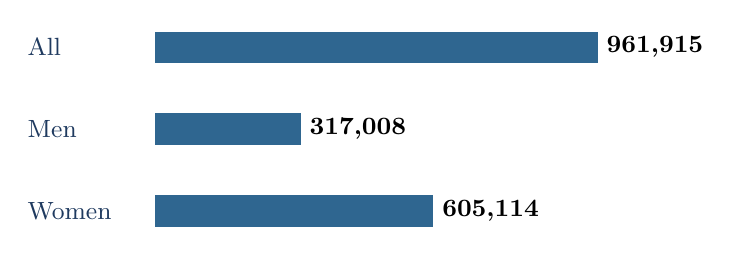
\begin{tikzpicture}[x=1cm,y=1cm,font=\small]
  \foreach \campaign/\y/\fraction/\exposures in {
    All/0/0.961915/{961,915}, Men/-1.04/0.317008/{317,008},
    Women/-2.08/0.605114/{605,114}} {
    \node[anchor=west,inner sep=0pt,text=navy] at (0,\y) {\campaign};
    \begin{scope}[xshift=1.62cm,x=5.85cm]
      \fill[accent] (0,\y-0.20) rectangle (\fraction,\y+0.20);
      \node[anchor=west,inner xsep=3pt,font=\small\bfseries] at (\fraction,\y) {\exposures};
    \end{scope}
  }
\end{tikzpicture}
\end{column}
\begin{column}{0.30\textwidth}
{\small\bfseries\color{navy} One model per item and display slot\par}
\vspace{2mm}
{\small Fit LinUCB and LogisticTS using user features and logged clicks.\par}
\vspace{4mm}
{\small Use the earliest 70\% of Random logs in each campaign, then freeze the fitted policies.\par}
\end{column}
\end{columns}
\note{I implemented and trained the two recommendation policies used in the evaluation. For each of our three campaigns, I used the earliest seventy percent of the Random logs as training data. All, the largest campaign, contains about nine hundred and sixty-two thousand training exposures. I fitted a separate model for each item and display slot.}
\end{frame}

\begin{frame}{How the two policies choose an item}
\begin{columns}[T,onlytextwidth]
\begin{column}{0.47\textwidth}
{\normalsize\bfseries\color{accent} LinUCB\par}
\vspace{1mm}
{\small Add an uncertainty bonus to predicted click reward. Choose the item with the highest score.\par}
\end{column}
\begin{column}{0.47\textwidth}
{\normalsize\bfseries\color{policyteal} LogisticTS\par}
\vspace{1mm}
{\small Use 64 posterior draws. Each item's win rate gives its selection probability.\par}
\end{column}
\end{columns}

\vspace{5mm}
{\small\bfseries\color{navy} Illustrative probabilities for one user and one slot\par}
\vspace{2mm}
\centering
\begin{tikzpicture}[x=1cm,y=0.66cm,font=\small]
  \foreach \offset/\barcolor/\patterns in {
    0/accent/{A/0/0/{0\%}, B/-1/1/{100\%}, C/-2/0/{0\%}},
    7.35/policyteal/{A/0/0.25/{25\%}, B/-1/0.625/{62.5\%}, C/-2/0.125/{12.5\%}}} {
    \begin{scope}[shift={(\offset,0)}]
      \foreach \itemName/\y/\fraction/\percentLabel in \patterns {
        \node[anchor=west,inner sep=0pt,text=navy] at (0,\y) {Item \itemName};
        \begin{scope}[xshift=1.55cm,x=3.57cm]
          \fill[navy!7] (0,\y-0.24) rectangle (1,\y+0.24);
          \fill[\barcolor] (0,\y-0.24) rectangle (\fraction,\y+0.24);
        \end{scope}
        \node[anchor=west,inner sep=0pt,font=\small\bfseries] at (5.27,\y) {\percentLabel};
      }
    \end{scope}
  }
\end{tikzpicture}
\note{The two methods handle uncertainty differently. LinUCB predicts click reward and adds an uncertainty bonus. The highest scoring item gets all the probability. Logistic Thompson Sampling fits a logistic click model. I fixed the random seed and used sixty-four draws from the approximate posterior. In this example, item B wins forty times, so its selection probability is sixty-two point five percent.}
\end{frame}

\begin{frame}{Twelve probability files for evaluation}
\begin{columns}[c,onlytextwidth]
\begin{column}{0.27\textwidth}
{\LARGE\bfseries\color{navy}12\par}
\vspace{1mm}
{\small\bfseries \texttt{.npy} files\par}
\vspace{2mm}
{\small One per policy, campaign, and test log.\par}
\end{column}
\begin{column}{0.69\textwidth}
{\small\bfseries\color{navy} Rows scored by each frozen policy\par}
\vspace{3mm}
{\small
\renewcommand{\arraystretch}{1.3}
\setlength{\tabcolsep}{0.8em}
\begin{tabular}{@{}lrr@{}}
\toprule
 & \textbf{Random/test} & \textbf{BTS/test} \\
 & \footnotesize IPS reference & \footnotesize OPE comparison \\
\midrule
All & 412,250 & 3,706,504 \\
Men & 135,860 & 1,223,053 \\
Women & 259,334 & 2,329,202 \\
\bottomrule
\end{tabular}\par}
\end{column}
\end{columns}
\vspace{5mm}
{\small\color{navy}
\textbf{Export checks} \quad Verified test row order and that probabilities sum to 1 per slot.\par}
\note{After training I froze both policies and scored each campaign's two test logs separately. That gave us twelve probability files. Each row contains the selection probabilities for every item at each of the three display slots. I checked the row order and verified that the probabilities sum to one at each slot.}
\end{frame}

\begin{frame}{Reference click rates on Random/test}
\centering
\begin{tikzpicture}[x=9.5cm,y=1cm,font=\small]
  \node[anchor=west,text=navy,font=\small\bfseries,inner sep=0pt] at (0,0.44) {Campaign};
  \draw[accent,thick] (0.21,0.44) -- (0.245,0.44);
  \fill[accent] (0.2275,0.44) circle[radius=2pt];
  \node[anchor=west,inner sep=2pt] at (0.25,0.44) {LinUCB};
  \draw[policyteal,thick] (0.43,0.44) -- (0.465,0.44);
  \fill[policyteal] (0.4475,0.44) circle[radius=2pt];
  \node[anchor=west,inner sep=2pt] at (0.47,0.44) {LogisticTS};
  \node[anchor=west,text=navy,font=\small\bfseries,inner sep=0pt] at (1.07,0.44) {IPS estimate};

  \foreach \tick in {0.2,0.4,0.6,0.8,1.0} {
    \draw[black!13] (\tick,-0.02) -- (\tick,-3.60);
    \node[below,inner sep=3pt,font=\footnotesize,text=black!72] at (\tick,-3.60) {\tick};
  }
  \draw[black!40] (0.2,-3.60) -- (1.0,-3.60);

  \foreach \campaign/\y in {All/-0.65, Men/-1.78, Women/-2.91} {
    \node[anchor=west,inner sep=0pt,text=navy,font=\small\bfseries] at (0,\y) {\campaign};
  }
  \foreach \y/\low/\value/\high/\barcolor in {
    -0.42/0.358/0.563/0.768/accent,
    -0.88/0.394/0.468/0.541/policyteal,
    -1.55/0.204/0.400/0.597/accent,
    -2.01/0.449/0.548/0.647/policyteal,
    -2.68/0.520/0.745/0.970/accent,
    -3.14/0.510/0.616/0.721/policyteal} {
    \draw[\barcolor,thick] (\low,\y) -- (\high,\y);
    \draw[\barcolor] (\low,\y-0.075) -- (\low,\y+0.075)
      (\high,\y-0.075) -- (\high,\y+0.075);
    \fill[\barcolor] (\value,\y) circle[radius=2.4pt];
    \node[anchor=west,text=\barcolor,inner sep=0pt,font=\small\bfseries] at (1.07,\y) {\value\%};
  }
  \node[font=\footnotesize,text=black!72] at (0.6,-4.24) {Estimated click rate (\%)};
\end{tikzpicture}\par
\vspace{1mm}
{\footnotesize Points mark IPS estimates. Lines show 95\% normal confidence intervals.\par}
\vspace{1mm}
{\footnotesize\bfseries\color{navy} On All, the paired 95\% interval for the difference includes zero.\par}
\note{The Random test log gives us a reference click rate through inverse propensity scoring. On All, the estimates are about zero point five six percent for LinUCB and zero point four seven percent for LogisticTS. The paired interval for the difference includes zero, so the ranking remains uncertain. The BTS probability files feed the estimation and clipping experiments my teammates will discuss next.}
\end{frame}
\endgroup

\begin{frame}{How we run the study}
\speak{
\item BTS rows inside the common test time window.
\item Sizes 1k to 20k, 50 repeats. Caps 1 to 1{,}000, plus no cap.
\item Policies frozen. Reward model refit by 3-fold cross-fitting each subset.
\item Error: MSE against the Random IPS reference $=$ bias$^2$ $+$ variance.
}
\end{frame}

\begin{frame}{Result 1: clipping}
\begin{center}
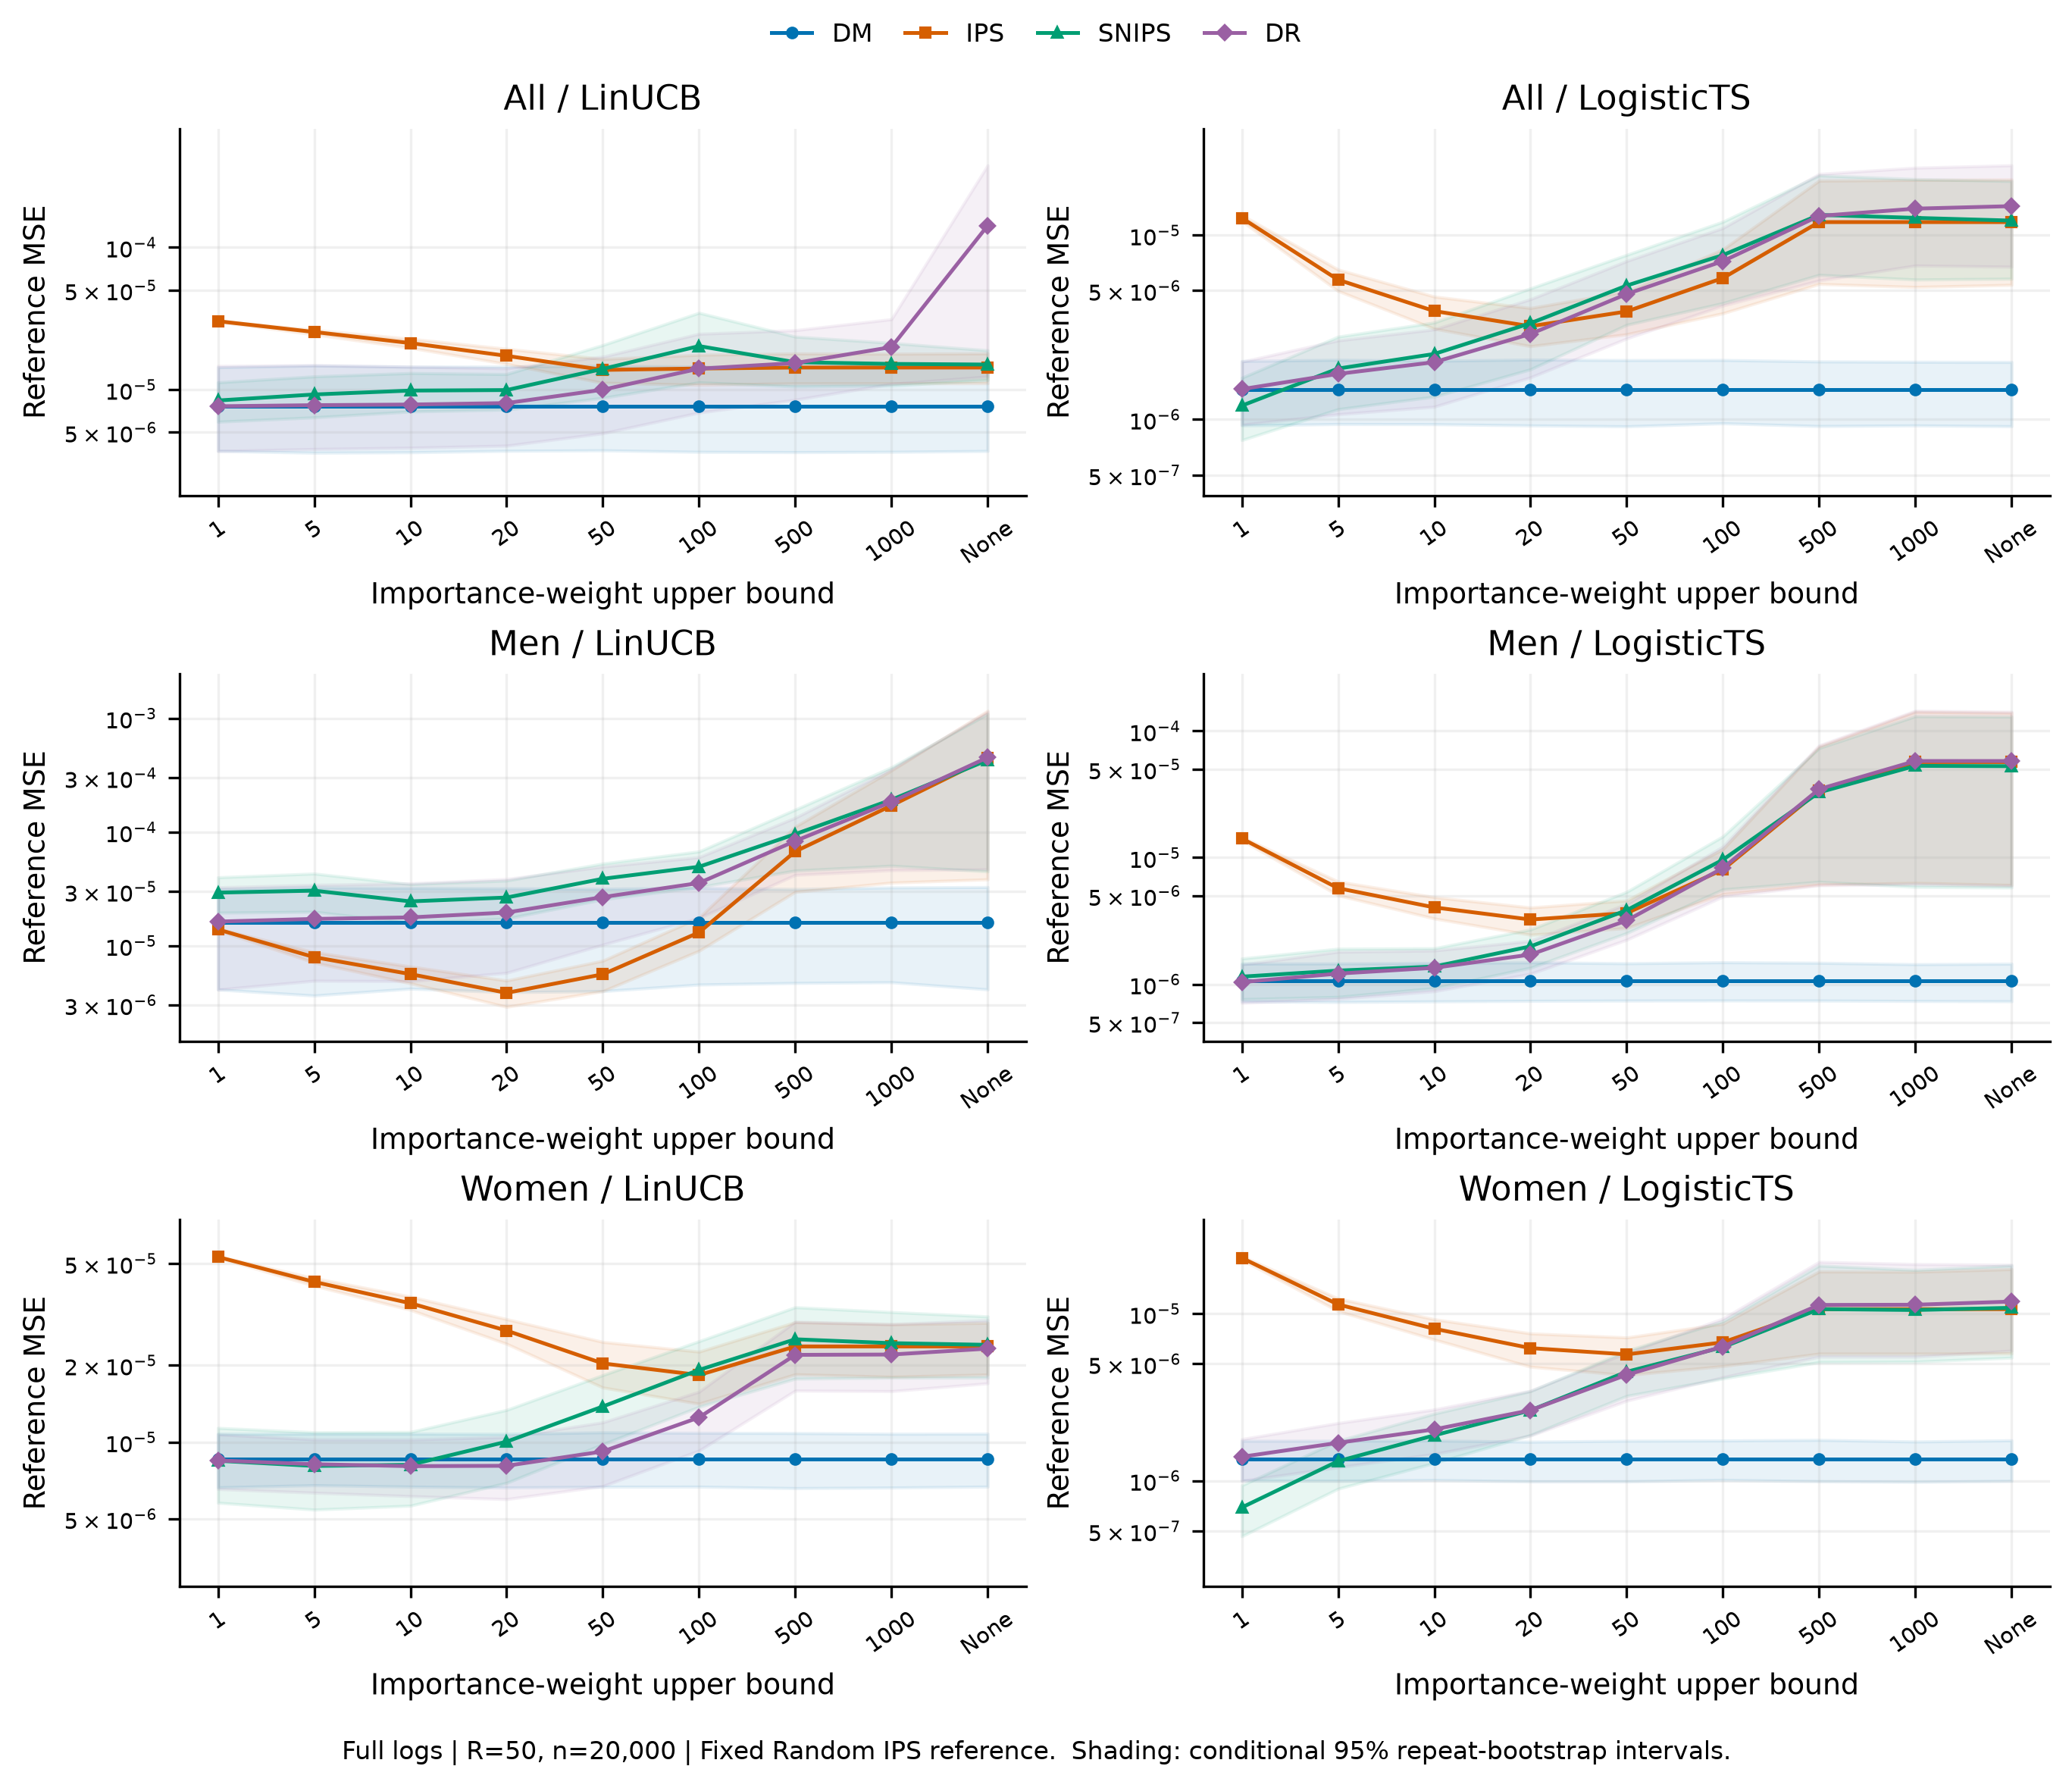
\includegraphics[width=0.98\textwidth,height=0.48\textheight,keepaspectratio]{clipping_mse_by_campaign.png}
\end{center}
\speak{
\item Main figure. X-axis: weight cap. Y-axis: reference MSE.
\item Panels: All, Men, Women. $n=20{,}000$, 50 repeats.
}
\end{frame}

\begin{frame}{What the clipping figure shows}
\speak{
\item DM is almost flat: it does not use the weights.
\item Unclipped IPS, SNIPS and DR sit much higher.
\item A small cap pulls those three toward DM. That is the bias--variance trade-off.
}
\end{frame}

\begin{frame}{Clipping numbers}
\begin{center}
\small
\begin{tabular}{llrr}
\toprule
All campaign & Cap & Unclipped DR MSE & Clipped DR MSE \\
\midrule
LinUCB & 1 & $1.42\times 10^{-4}$ & $7.63\times 10^{-6}$ \\
LogisticTS & 1 & $1.44\times 10^{-5}$ & $1.46\times 10^{-6}$ \\
\bottomrule
\end{tabular}
\end{center}
\vspace{2mm}
\speak{
\item Cap 1 cuts All DR reference MSE by \textbf{94.6\%} (LinUCB) and \textbf{89.8\%} (LogisticTS).
\item Then the DR to DM ratio on All is about 1. Clipping is not free.
\item Women / LinUCB: best cap is 10, not 1.
}
\end{frame}

\begin{frame}{A few rows dominate the weights}
\begin{columns}[T]
\begin{column}{0.50\textwidth}
\speak{
\item All LinUCB: unclipped $\mathrm{ESS}/n$ is only 0.23\%.
\item Cap 1 throws away about 97\% of the weight mass.
\item Most IPS mass came from a few extreme rows.
\item Best caps were chosen on the same reported grid.
}
\end{column}
\begin{column}{0.48\textwidth}
\centering
\art{huge-weight.jpg}
\end{column}
\end{columns}
\end{frame}

\begin{frame}{Result 2: sample size}
\begin{center}
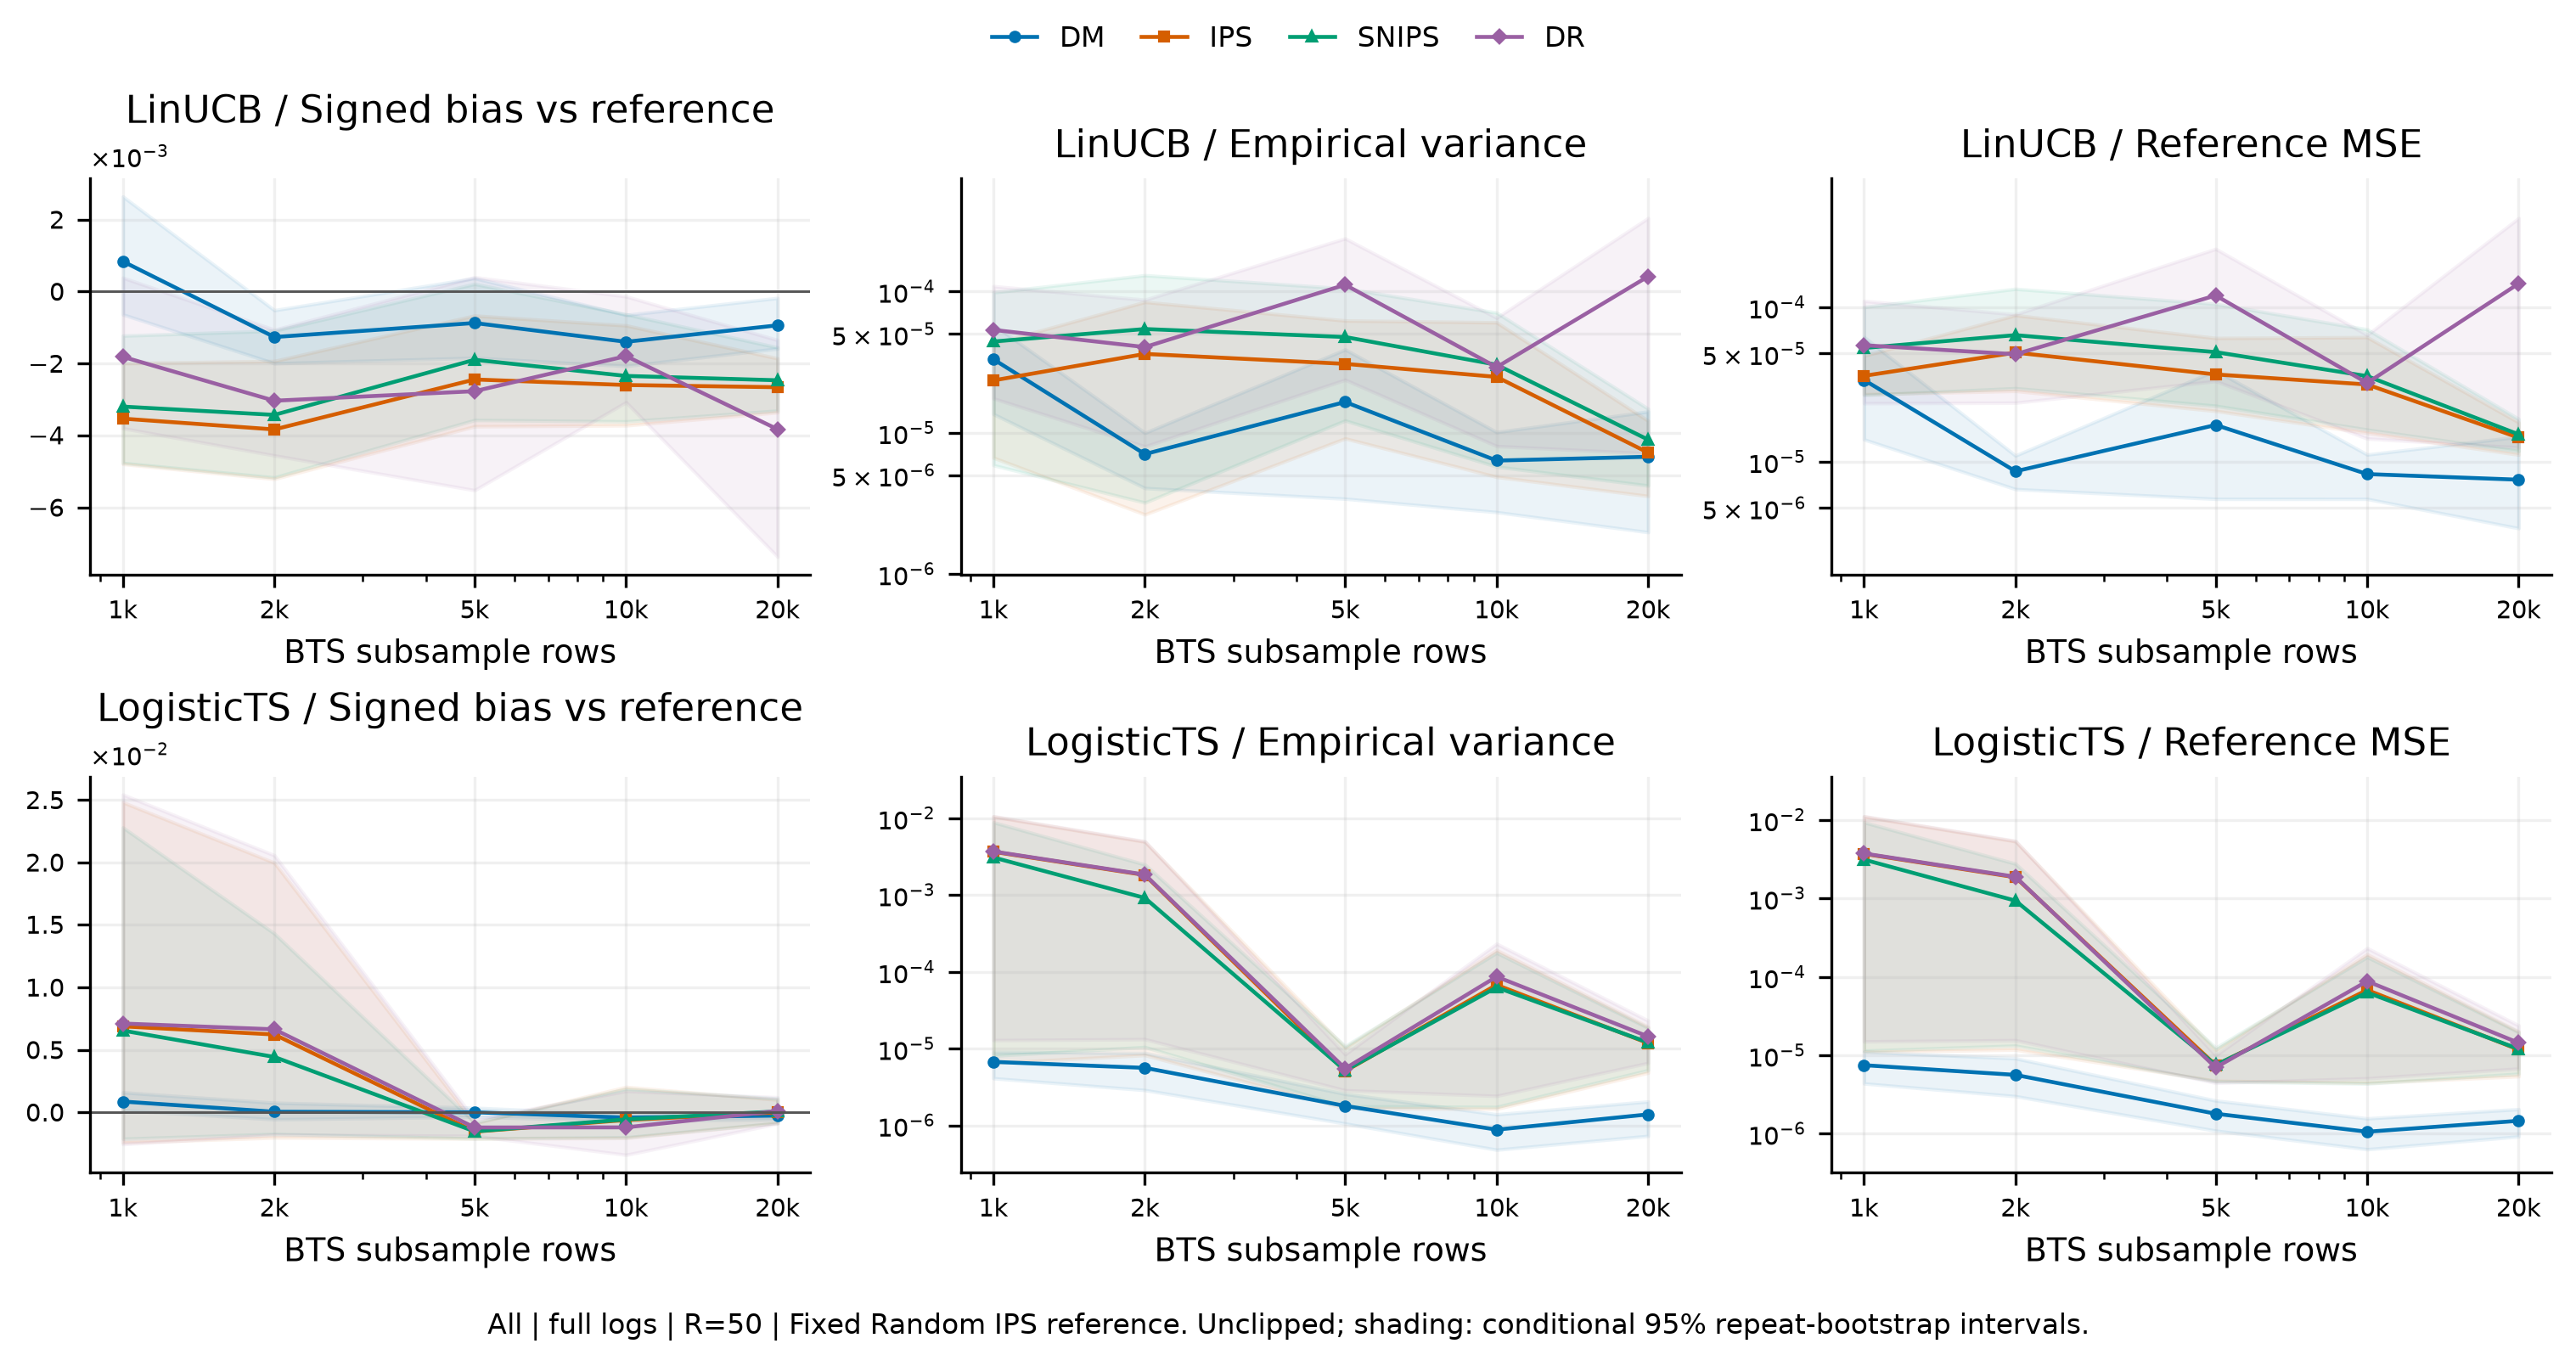
\includegraphics[width=0.95\textwidth,height=0.48\textheight,keepaspectratio]{sample_size_all.png}
\end{center}
\speak{
\item All campaign, both policies. Top: LinUCB. Bottom: LogisticTS.
\item Columns: bias, variance, reference MSE. Unclipped.
}
\end{frame}

\begin{frame}{More data does not always help}
\speak{
\item LogisticTS: unclipped DR error falls as $n$ grows.
\item LinUCB: unclipped DR error can \textbf{rise} with $n$, because a larger sample is more likely to hit one huge weight.
\item More data does not automatically fix IPS-family estimators when overlap is poor.
}
\end{frame}

\begin{frame}{Result 3: ranking}
\begin{columns}[T]
\begin{column}{0.56\textwidth}
\begin{center}
\scriptsize
\begin{tabular}{lrrrr}
\toprule
Unclipped & DM & DR & IPS & SNIPS \\
\midrule
All & 48\% & 32\% & 30\% & 30\% \\
Men & 58\% & 52\% & 52\% & 44\% \\
Women & 38\% & 42\% & 44\% & 48\% \\
\bottomrule
\end{tabular}
\end{center}
\vspace{2mm}
\speak{
\item On All, DM agrees 48\% of the time. The others are about 30\%.
\item Close to a coin flip, because the reference order is uncertain.
}
\end{column}
\begin{column}{0.42\textwidth}
\centering
\art[0.98\linewidth]{coin-flip-ranking.jpg}\\[1mm]
{\scriptsize Uncertain ranking.}
\end{column}
\end{columns}
\end{frame}

\begin{frame}{Takeaways and strengths}
\speak{
\item Unclipped IPS-family estimators are dominated by rare large weights.
\item Clipping stabilizes DR, but then DR tracks DM.
\item We cannot confidently rank LinUCB versus LogisticTS.
\item Strengths: real industrial logs, a bounded Random reference, frozen policies, reproducible pipeline.
}
\end{frame}

\begin{frame}{Limits and extensions}
\speak{
\item Limits: sparse clicks, weak LinUCB overlap, noisy Random reference, only two policies, same-grid clipping minima.
\item Switch-DR was poster outlook. We did not implement it.
\item Extensions: Switch-DR or shrinkage, more stochastic policies, session-level bootstrap.
}
\end{frame}

\begin{frame}[plain]
\centering
\vspace{22mm}
{\Large\bfseries\color{navy} Thank you\par}
\vspace{8mm}
{\large Questions\par}
\vspace{12mm}
{\small Group 7 \quad City University of Hong Kong (Dongguan)\\[1mm]
visual layout trial}
\end{frame}

\end{document}
